\documentclass[a4paper,12pt]{report}
\usepackage[spanish,mexico]{babel}
\usepackage[utf8]{inputenc}
\usepackage[T1]{fontenc}
\usepackage{amsmath}
\usepackage{amssymb}
\usepackage{wasysym}
\usepackage[dvipsnames,pdftex]{color}
\usepackage[colorinlistoftodos]{todonotes}
\usepackage[left=3.0cm,right=1.0cm,top=2.0cm,bottom=2cm]{geometry}
%\usepackage{helvet}
%\renewcommand{\familydefault}{\sfdefault}
\setlength{\oddsidemargin}{0in}
\usepackage{float}
 %\setlength{\textwidth}{6in}
 \setlength{\topmargin}{0in}
 \setlength{\voffset}{-0.1in}
 \setlength{\hoffset}{0.2in}
 \setlength{\textheight}{9.7in}
 \setlength{\textwidth}{6.5in}
 \setlength{\topskip}{0in}
 \setlength{\parskip}{2ex}
 \renewcommand{\baselinestretch}{1}
\usepackage{diagbox}
\usepackage{verbments}
\usepackage{verbatim}
\definecolor{fondo1}{rgb}{0.9, 0.9, 0.9}
\definecolor{fondo2}{rgb}{0.1647, 0.4980, 0.1}
\usepackage{array}
\usepackage{listings}
%\useapackage{caption}
%%% comandos definidos por el usuario

\begin{document}
\fvset{frame=bottomline, framerule=0.02cm,numbers=left, numbersep=8pt}
\plset{language=c++,texcl=true, listingnamefont=\sffamily\bfseries\color{white},captionbgcolor=fondo2, bgcolor=fondo1,listingname=\textbf{Programa}, captionfont=\sffamily\color{white}}
\setcounter{page}{1}
\pagenumbering{roman}
\thispagestyle{empty}
\begin{center}
{\huge UNIVERSIDAD NACIONAL DE INGENIERÍA}\\[0.9cm]
{\Large FACULTAD DE INGENIERÍA MECÁNICA}\\[0.6in]
\end{center}
\begin{figure}[h]
\begin{center}

\includegraphics[scale=0.33]{logoUNI.png}
%\vspace{0cm}
\end{center}
\end{figure}
\vspace{0.4cm}
\begin{center}
CIRCUITOS ELECTRICOS\\[14mm]
{\Large CIRCUITOS TRANSITORIOS\\ Y RECTIFICACIÓN DE ONDAS}\\[10mm]
\vfill
LIMA - PERÚ \hfill JULIO 2019
\end{center}
\newpage
\thispagestyle{empty}
\begin{center}
{\LARGE CIRCUITOS TRANSITORIOS\\ Y RECTIFICACIÓN DE ONDAS}\\[0.7cm]
\small ENTREGADO:\\[0.3cm]
\small 04 JULIO 2019\\[0.9cm]
\end{center}
\begin{flushleft}
{\large INTEGRANTES:}\\[3cm]
\end{flushleft}
%\begin{tabular}{c@{\hspace{0.5in}}c}
%\rule[1pt]{2.6in}{1pt}&\rule[1pt]{2.6in}{1pt}\\
%Huaroto Villavicencio Josué, 20174070I & Maguiña Amaya Wladimir, 20172019F\\[2.5cm]
%\rule[1pt]{2.6in}{1pt}&\rule[1pt]{2.6in}{1pt}\\
%Perez La Rosa Fabrizio, 20170234G & Seclén Yberos Carlos, 20174137F\\[2.5cm]
%\rule[1pt]{2.6in}{1pt}&\rule[1pt]{2.6in}{1pt}\\
%Saravia Echevarria Henrry, 20170233K & Sotelo Cavero Sergio, 20172125K\\[2.5cm]
%\end{tabular}
%\begin{center}
%\begin{tabular}{c@{\hspace{0.5in}}c}
%\rule[1pt]{3.14in}{1pt}\\UE
%Sotelo Cavero Sergio, 20172125K% & Nombre 5, 2017 \\[1.5cm]
%\end{tabular}
%\end{center}
\begin{center}
\begin{tabular}{c@{\hspace{0.5in}}c}
\rule[1pt]{3.14in}{1pt}\\
Huaroto Villavicencio Josué, 20174070I \\[3cm]
\rule[1pt]{3.14in}{1pt}\\
Quesquen Vitor Angel, 20172019F \\[3cm]
\rule[1pt]{3.14in}{1pt}\\
Landeo Sosa Bruno, 19774147I \\[3cm]
\rule[1pt]{3.14in}{1pt}\\
Sotelo Cavero Sergio, 20172125K
\end{tabular}
\end{center}
%\\[0.7cm]
{\large PROFESOR:} \\[1.3cm]
\begin{center}
\begin{tabular}{c}
\rule[3pt]{4.8in}{1pt}\\[1pt]
ING. Tarazona Bermúdez, Bernabé
\end{tabular}
\end{center}
\vfill
%\newpage
%\begin{center}
%{\Large \bf{RESUMEN}}
%\end{center}
\newpage
\begin{abstract}
El presente trabajo es una comprobación de los fenómenos estudiados en la parte teórica del curso. Para ello, se utilizó los instrumentos disponibles del laboratorio de automatización de la facultad de ingeniería mecánica.
\end{abstract}
\tableofcontents
\listoffigures
\addcontentsline{toc}{chapter}{Índice de Figuras}
\chapter{Objetivos}
\begin{enumerate}
\item Familiarizarse con los instrumentos de medición del laboratorio de automatización.
\item Aprender mediante la experiencia el funcionamiento y comportamiento de los diversos elementos electricos y electronicos.
\item Observar los cuidados requeridos para cada instrumento.
\item Comparar el comportamiento teórico con el real de las distintas distribuciones usadas en la experiencia.
\end{enumerate}
\pagenumbering{arabic} %%% esto es para regresar el modo de numeración a numeración arábiga
\setcounter{page}{1}  %%% empezamos en página 1
\chapter{Circuitos transitorios}
La respuesta natural de un circuito con un resistor, un inductor y un capacitor (\text{RLC)} puede tomar tres formas diferentes, dependiendo de los valores específicos de sus componentes. La ecuación característica del circuito RLC es:
$$
s^{2} + \frac{R}{L}s + \frac{1}{LC} = 0
$$
$$
s = \frac{-R \pm \sqrt{R^{2} - 4L/C}}{2L}
$$
Por comodidad definimos las variables $\alpha$ y $\omega$ como $\frac{R}{2L}$ y $\frac{1}{\sqrt{LC}}$ respectivamente. Donde $\alpha$ se llama factor de amortiguamiento y $\omega$ es la frecuencia de resonancia. Dependiendo de los tres casos se presentan distintas soluciones:
\begin{enumerate}
\item \textbf{Sobreamortiguado.} Si $\alpha > \omega$
\item \textbf{Críticamente amortiguado.} Si $\alpha = \omega$
\item \textbf{Subamortiguado.} Si $\alpha < \omega$
\end{enumerate}
Siendo las soluciones:
\begin{enumerate}
\item \textbf{Sobreamortiguado}
$$
v_{(t)} = A_{1}e^{s_{1}t} + A_{2}e^{s_{2}t}
$$
\item \textbf{Críticamente amortiguado}
$$
v_{(t)} = A_{1}te^{-\alpha t} + A_{2}e^{-\alpha t}
$$
\item \textbf{Subamortiguado}
$$
v_{(t)} = B_{1}e^{-\alpha t}\cos \omega t + B_{2}e^{-\alpha t}\sin \omega t
$$
\end{enumerate}
\section{Materiales}
Para encontrar los valores de resistencias, capacitancias e inductancias para generar los 3 casos utilizamos el siguiente código escrito en C++ y Python:
\begin{comment}
\begin{pyglist}[language=c++,caption={C++},listingname={\textbf{Circuito transitorio}},style=perldoc]
#include <bits/stdc++.h> 
using namespace std; 
int main(){ 
float aux1 = 1,aux2 = -1;
int firstansw = 0,secondansw = 0,thirdansw = 0;
int answ1 = 0;
int answ2 = 0;
int answ3 = 0;
int res[6] = {10000,6800,2150,100,200,4950};
float cap[4] = {10,100,4.7,2.2};
float ind[4] = {20,0.001,0.01,0.0047};
for(int i=0; i<6; i++){
  for(int j=0; j<4; j++){
    for(int k=0; k<4; k++){
      float alpha = 500.0*res[i]/ind[k];
      float omega = 1000000.0/sqrt(1.0*ind[k]*cap[j]);
      if(abs(alpha-omega)<0.1){
        cout<<"Criticamente amortiguado:\n";        
        cout<<res[i]<<"Ohm "<<cap[j]<<"nF "<<ind[k]<< "mH\n";
      }
      if(alpha-omega < 0){
        if(aux1 > alpha-omega){
          aux1 = alpha-omega,firstansw = i,secondansw = j,thirdansw = k;         	
        }
      }
      if(alpha-omega > 0){
        if(aux2 < alpha - omega){
          aux2 = alpha-omega,answ1 = i,answ2 = j,answ3 = k;
        }
      }
    }		
  }	
}
cout<<"Subamortiguado:\n";
cout<<res[firstansw]<<"Ohm "<<cap[secondansw]<<"nF "<<ind[thirdansw]<<"mH\n";
cout<<"Sobreamortiguado:\n";
cout<<res[answ1]<<"Ohm "<<cap[answ2]<<"nF "<<ind[answ3]<<"mH\n";
return 0; 
}
\end{pyglist}
\newpage
\begin{pyglist}[language=python,caption={Python},listingname={\textbf{Circuito transitorio}},style=tango]
import math
aux1 = 0
aux2 = -1
res = [10000,6800,2150,100,200,4950]
cap = [10,100,4.7,2.2]
ind = [20,0.001,0.01,0.0047]
for i in range(0,6):
    for j in range(0,4):
        for k in range(0,4):
            alpha = 500*res[i]/ind[j];
            omega = 1000000*math.sqrt(ind[k]*cap[j]);
            if abs(alpha-omega)<0.1:
                print("Criticamente amortiguado:")
                print(res[i],"Ohm",cap[j],"nF",ind[k],"mH")
            if alpha-omega < 0:
                if aux1 > alpha-omega:
                    aux1 = alpha-omega
                    firstansw = i
                    secondansw = j
                    thirdansw = k
            if alpha-omega > 0:
                if aux2 < alpha-omega:
                    aux2 = alpha-omega
                    answ1 = i
                    answ2 = j
                    answ3 = k
print("Subamortiguado:")
print(res[firstansw],"Ohm",cap[secondansw],"nF",ind[thirdansw],"mH")
print("Sobreamortiguado:")
print(res[answ1],"Ohm",cap[answ2],"nF",ind[answ3],"mH")
\end{pyglist}
\end{comment}
Ambos códigos arrojan como salida:\\
%Criticamente amortiguado:\\
%20 Ohm 100nF 0.01mH\\
Subamortiguado:\\
100 Ohm \hspace{10pt} 2.2nF \hspace{10pt} 0.01mH\\
Sobreamortiguado:\\
10000 Ohm \hspace{10pt} 100nF \hspace{10pt} 0.001mH\\
El valor de críticamente amortiguado no es obtenido, pero al hacer un acoplamiento en paralelo de las resistencias de 6.8$\,$kOhm y 10$\,$kOhm con 4.7$\,$nF y 20$\,$mH se obtiene un comportamiento cercano al críticamente amortiguado:
$$
\alpha = 101190 \hspace{20pt} \omega = 103142 \longrightarrow \frac{\alpha - \omega}{\omega} \cdot 100\% = 1.928689\%
$$
Críticamente amortiguado:\\
6.8$\,$kOhm + 10$\,$kOhm \hspace{10pt} 4.7$\,$nF \hspace{10pt} 20$\,$mH
\section{Comprobación experimental}
\subsection{Subamortiguado}
Con la configuración de 100$\,$Ohm, 2.2$\,$nF y 10$\,\mu$H.
Con la configuración de 10$\,$kOhm, 100$\,$nF y 1$\,\mu$H.
\begin{figure}[H]
\begin{center}
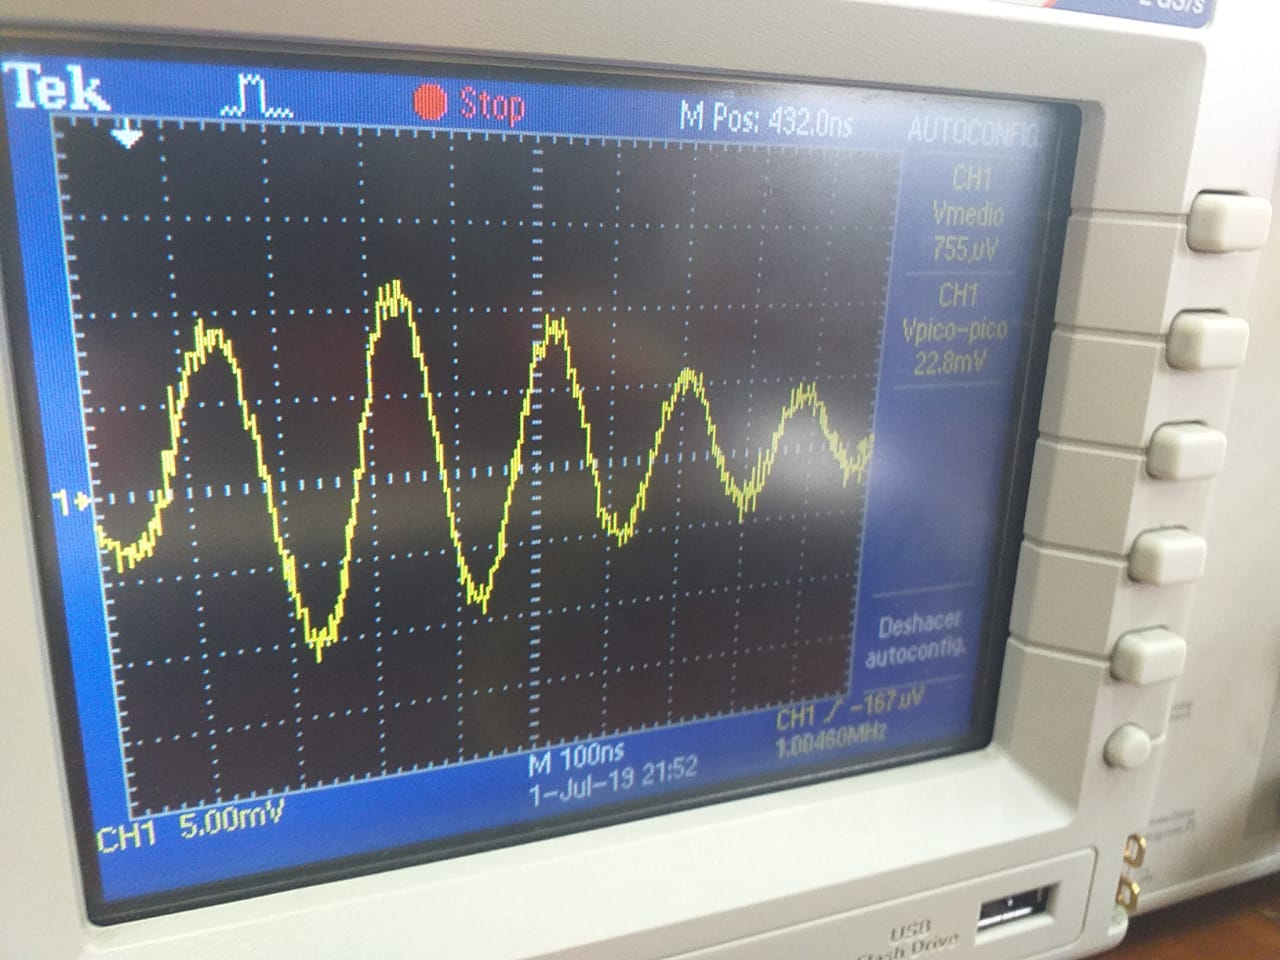
\includegraphics[scale=0.24]{sub.jpeg}
\end{center}
\end{figure}
\subsection{Sobreamortiguado}
Con la configuración de 10$\,$kOhm, 100$\,$nF y 1$\,\mu$H.
\begin{figure}[H]
\begin{center}
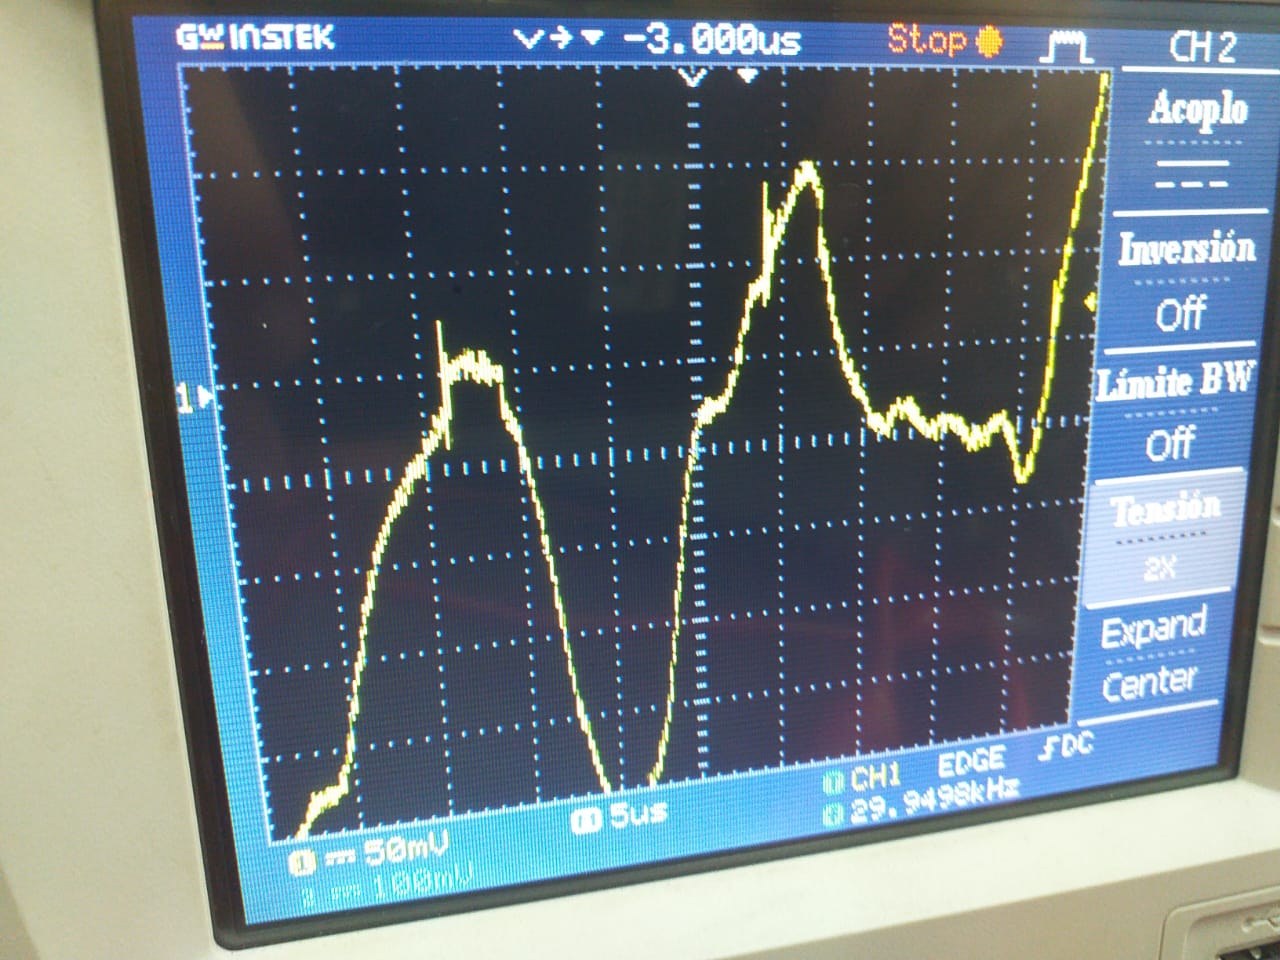
\includegraphics[scale=0.24]{sob.jpeg}
\end{center}
\end{figure}
\subsection{Críticamente amortiguado}
Con la configuración de 10$\,$kOhm y 6.8$\,$kOhm en paralelo, 4.7$\,$nF y 20$\,$mH.
\begin{figure}[H]
\begin{center}
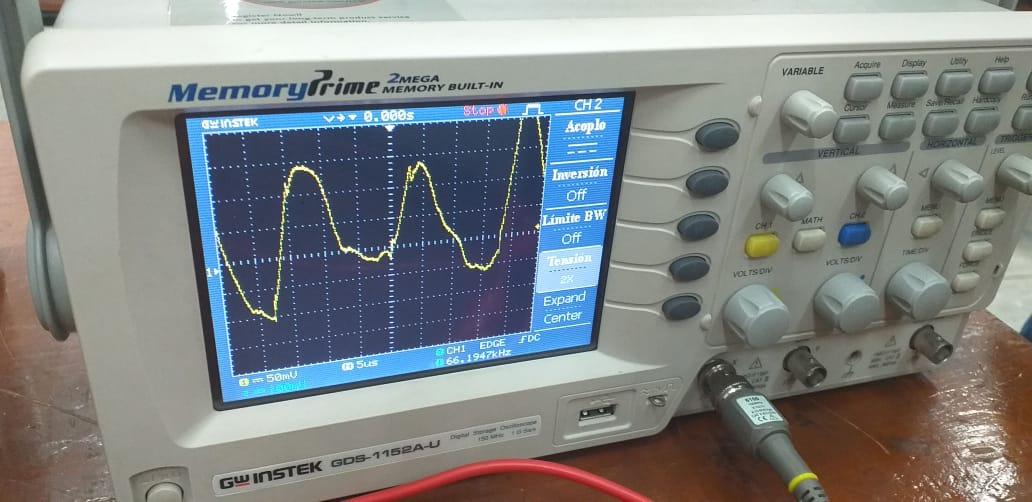
\includegraphics[scale=0.33]{crit.jpeg}
\end{center}
\end{figure}
\newpage
\section{Justificación del error experimental}
Observamos en las imágenes del osciloscopio que la forma de la onda no es muy parecida a los resultados teóricos. El error puede deberse a que a menudo es muy difícil conseguir un comportamiento críticamente amortiguado, sin embargo; lo ideal podría ser muy cercano; ello se observa en nuestro porcentaje de error que es menor al 2\%. La interferencia y las medidas que nos da el generador de corriente continua también pueden ser un factor que altera la gráfica del osciloscopio, pues se observa un comportamiento errático en el tiempo; lo que indica que no ha estado recibiendo una cantidad constante de voltaje. Las gráficas entonces coinciden con la solución esperada al considerar fuentes de corriente alterna. La explicación para esto es sencilla; los valores de inductancia son muy pequeños y para conseguir comportamientos sobreamortiguados y críticos fue necesario usar valores muy pequeños de resistencias y capacitancias; haciendo el comportamiento de la corriente más sensible al cambio de voltaje que podría entregarnos la fuente; así una pequeña interferencia entre la fuente y el circuito armado produce grandes cambios sinusoidales en la gráfica mostrada por el osciloscopio.
\chapter{Rectificación de ondas}
\section{Rectificación de media onda}
Para la rectificación de media onda solo es necesario un diodo, estos elementos son capaces de cambiar la forma de señal de la onda en la entrada. En este caso el diodo elimina la mitad de la señal que recibe en la entrada, en función de como este polarizado el diodo; si la polarización es directa, se elimina la parte negativa de la señal, y si la polarización es inversa se elimina la parte positiva de la señal. Al momento de rectificar en media onda es necesario tener en cuenta los siguientes parámetros:
\begin{center}
\begin{tabular}{|c|c|c|}
\hline 
Parámetro & Fórmula & Observaciones \\ 
\hline 
Valor medio de la tensión & $\displaystyle  V_{med} = \frac{V_{max}}{\pi}$ & Es la media aritmética de todos los \\
& & valores instantáneos de la señal\\
& & comprendidos en un intervalo.\\
\hline 
Valor eficaz de la tensión & $\displaystyle  V_{ef} = \frac{V_{max}}{2}$ & Este valor de tensión lo podemos \\
& & comprobar con un polímero \\ 
\hline 
Valor medio de la intensidad & $\displaystyle I_{med} = \frac{V_{med}}{R}$ & Se obtienen aplicando la ley de Ohm \\ 
\cline{1-2} 
Valor eficaz de la intensidad & $\displaystyle V_{ef} = \frac{V_{ef}}{R}$ & a los valores de la tensión \\ 
\hline 
\end{tabular} 
\end{center}
\subsection{Materiales}
\begin{enumerate}
\item 1 resistencia de 2.15$\,$kOhm
\item 1 diodo 1N5399 LD, Máximo 1$\,$A
\item Osciloscopio
\item Generador de ondas
\item Cables de conductores
\end{enumerate}
\subsection{Experiencia}
\begin{enumerate}
\item Con ayuda de los cables formamos el circuito conformado por el diodo y el resistor.
\item Conectamos la sonda del osciloscopio a los extremos de la resistencia de tal manera que el positivo quede entre el diodo y la resistencia, el negativo estará en el otro extremo.
\item Para este primer arreglo se tendrá en el osciloscopio una media onda donde se eliminaron los ciclos negativos. Se elige la escala adecuada y se comprueban los valores.
\end{enumerate}
\subsection{Polarización directa}
Para 12$\,$V, 2.15$\,$kOhm, 1 diodo:
$$
V = V_{ef}\sqrt{2}\cdot \sin \omega t
$$
La corriente que pasa por la carga es:
$$
I_{ef} = \frac{V_{ef}}{R} = \frac{12\sqrt{2}}{2150} = 0.0008\,\mathrm{A}
$$
Este valor es menor que 1A , por lo tanto el diodo no excederá su límite.\\
La tensión entre los bornes de la resistencia es corregida por el diodo, quedando de la siguiente manera:
\begin{figure}[H]
\begin{center}
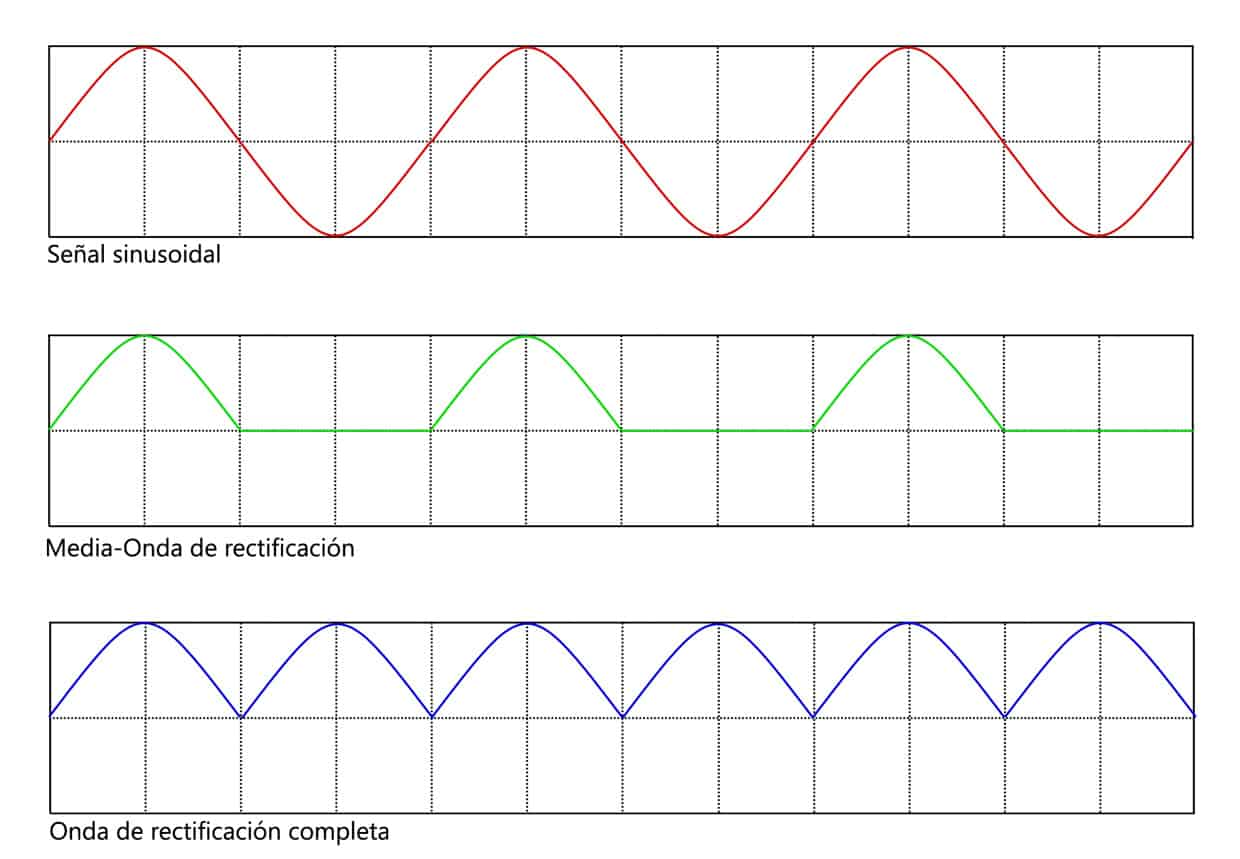
\includegraphics[scale=0.35]{cir.jpg}
\caption{Rectificación de ondas}
\end{center}
\end{figure}
La señal de la onda es modificada eliminando los ciclos negativos, debido a la posición del diodo con respecto a la fuente. Teóricamente el valor máximo debe ser el mismo, pero el diodo no es un elemento ideal, por lo que produce una ligera caída de tensión de aproximadamente 0.7V.
\begin{figure}[H]
\begin{center}
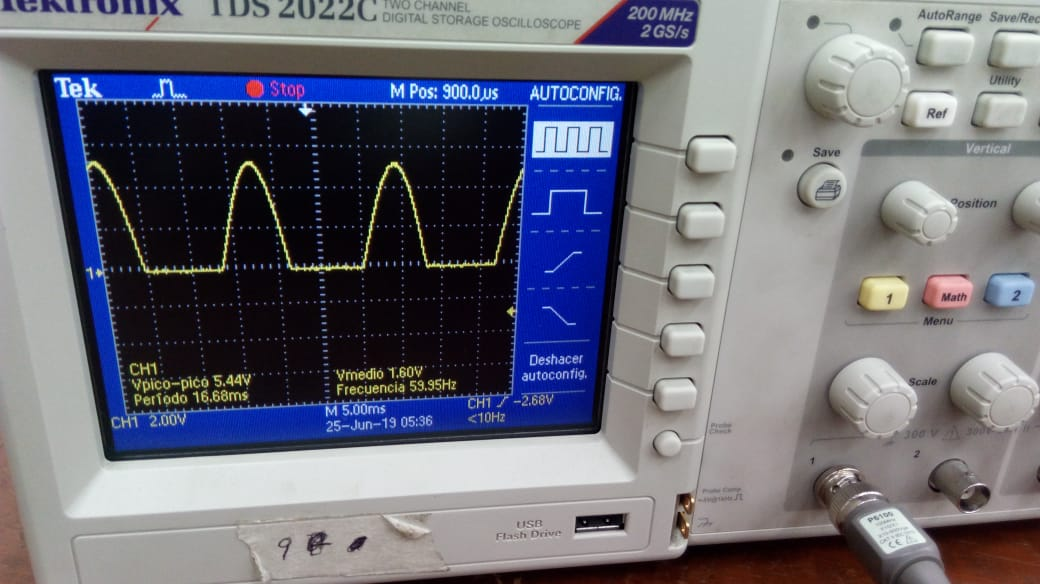
\includegraphics[scale=0.4]{circ1.jpg}
\caption{Osciloscopio mostrando la rectificación}
\end{center}
\end{figure}
\begin{figure}[H]
\begin{center}
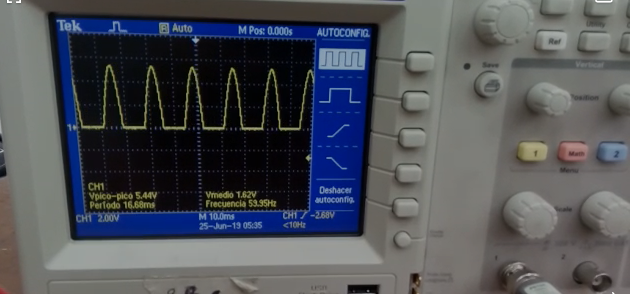
\includegraphics[scale=0.7]{circ3.jpg}
\caption{Osciloscopio mostrando la rectificación}
\end{center}
\end{figure}
\begin{figure}[H]
\begin{center}
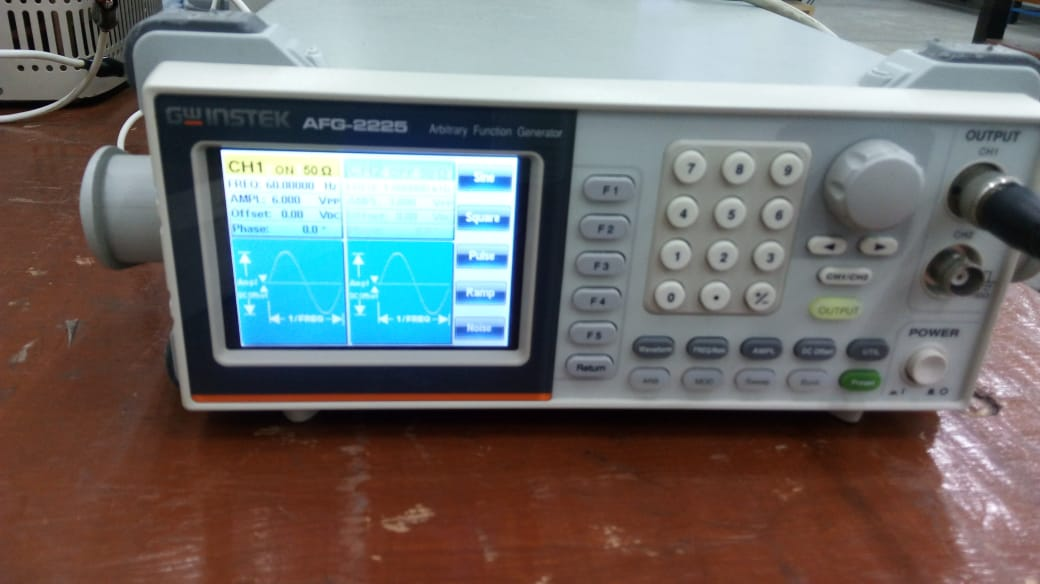
\includegraphics[scale=0.45]{circ2.jpg}
\caption{Generador de ondas}
\end{center}
\end{figure}
\begin{figure}[H]
\begin{center}
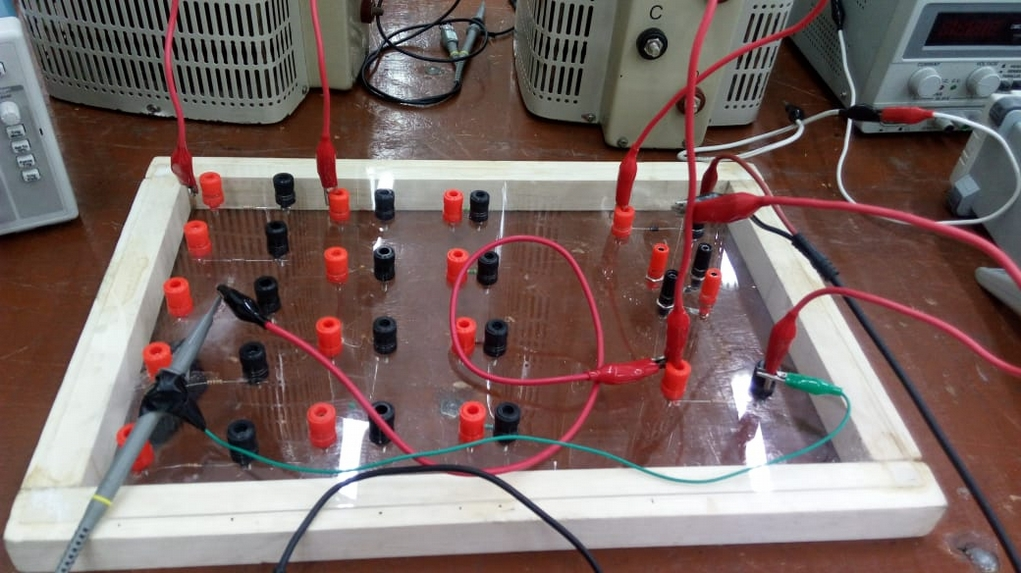
\includegraphics[scale=0.45]{circ4.jpg}
\caption{Trabajo realizado para la comprobación experimental}
\end{center}
\end{figure}
\section{Rectificador de onda completa}
El circuito rectificador de onda completa es el más empleado para la alimentación de los equipos electrónicos. En nuestro caso usaremos un puente de diodos para rectificar.
\subsection{Materiales}
\begin{itemize}
\item 1 resistencia de 2.15$\,$kOhm
\item 1 puente de diodos W08, máximo 1$\,$A
\item Osciloscopio
\item Generador de ondas
\item Cables conductores
\subsection{Experiencia}
\begin{enumerate}
\item Con ayuda de los cables formamos el circuito conformado por el puente de diodos y el resistor.
\item Conectamos la sonda del osciloscopio a los extremos de la resistencia donde se recibe la onda rectificada.
\item Para esta experiencia se obtiene en el osciloscopio una onda completa rectificada, donde los ciclos negativos se convirtieron en positivos. Se elige la escala adecuada y se comprueban los valores.
\end{enumerate}
\end{itemize}
\begin{figure}[H]
\begin{center}
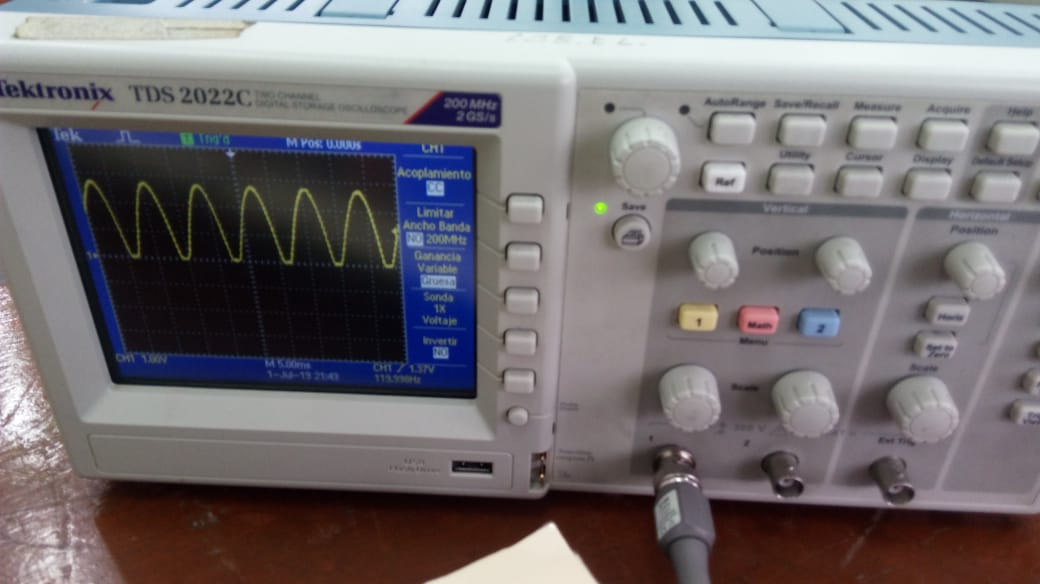
\includegraphics[scale=0.42]{kesk2.jpeg}
\caption{Rectificación de onda completa}
\end{center}
\end{figure}
\begin{figure}[H]
\begin{center}
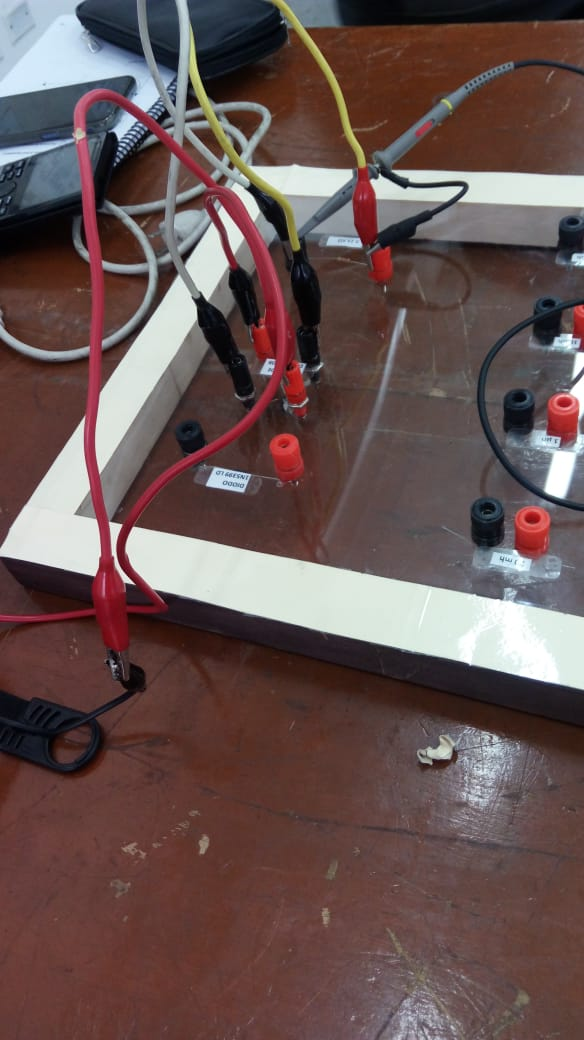
\includegraphics[scale=0.42]{kesk3.jpeg}
\caption{Conexión para la rectificación de ondas}
\end{center}
\end{figure}
\chapter*{Conclusiones}
\addcontentsline{toc}{chapter}{Conclusiones}
\begin{enumerate}
\item Se comprueba el funcionamiento del diodo cuando se hace pasar una corriente con funcion de onda sinusoidal y esta es modificada quedando solo las partes positivas o las negativas segun la orientacion del diodo.
\item El puente de diodos es el resultado de acoplar diodos con el fin de modificar la forma de la onda y hacerla mas estable.
\item Se concluye que en circuitos RC y RL el aumento de la frecuencia es una buena opción para modificar el desfase.
\item El régimen transitorio de un circuito solo puede ser subamortiguado, sobreamortiguado o críticamente amortiguado.
\item El régimen transitorio nos indica como fluctua la corriente a través del tiempo antes de llegar a ser estable.
\item Concluimos en que SerGod no nos pasó conclusiones.
\item Lo mismo que el de arriba :v.
\end{enumerate}
\begin{thebibliography}{99}  %%%este es un contador para el número de bibliografías utilizados.
\addcontentsline{toc}{chapter}{Bibliograf\'{\i}a} %%% Para introducir la bibliografía en el índice.
%\bibitem{Rahman}{Rahman,Aminur y Doe, Hidekazu; ``Ion transfer of tetraalkylammonium cations at an interface between 
%frozen aqueous solution and 1,2-dichloroethane".{\em{Journal of Electroanalytical Chemistry}} {\bfseries 424},159,(1997).}
%\bibitem{Martins}{Martins, M.C., Pereira, C.M., Girault,H.H y Silva, F.; ``Specific adsorption of tetraalkylammonium 
%cations on the 1,2-dichloroethane/water interface".{\em{Electrochimica Acta}} {\bfseries 50},135,(2004).}
%\bibitem{Ding}{Ding, Zhifeng. ``Spectroelectrochemistry and photoelectrochemistry of charge transfer at liquid/liquid
%interfaces". {\em {Tesis, EPFL,}}(1999).}
%\bibitem{IR}{Princeton Applied Research. \em{Technical Note 101}}
%\bibitem{Beni}{Beni V., Ghita M. y Arrigan D. ``Cyclic and pulse voltammetric study of dopamine at the interface between
%two inmiscible electrolyte solutions". {\em{Biosensors \& Biolectronics}} {\bfseries 20}, 2097, (2005).}
%\bibitem{Samec2}{Samec Z., Lhotsky A., Jänchenová H., y Marecek, V. ``Interfacial tension and impedance measurements
%of interfaces between two inmiscible electrolyte solutions". {\em{Journal of Electroanalytical Chemistry}} {\bfseries
%43}, 47, (2000).}
%\bibitem{Day}{Day R.A. y Underwood A.L. {\textit{Química Analítica Cuantitativa}},5ºed. Prentice-Hall, México, 1998. 45-48.}
\bibitem{Boylestad}{Boylestad, Robert L. ``Introducción al análisis de circuitos''. {\em{Pearson.}}}
\bibitem{Sadiku}{Sadiku, Matthew N. y Alexander, Charles K. ``Fundamentos de circuitos eléctricos''.{\em{Mc Graw Hill}}}
\bibitem{Zill}{Zill, Dennis G. ``Ecuaciones diferenciales con aplicaciones de modelado''.{\em{Thomson}}}
%\bibitem{Dieter}{Dieter. ``Metalurgia mecánica''.}
%\bibitem{Apraiz}{Apraiz, J. ``Tratamiento Térmico de los Aceros''.}
%\bibitem{Smith}{Smith, William F. y Ph.D. Hashemi, Javad ``Ciencia e ingeniería de materiales". {\em{
%Madrid: McGraw-Hill, Interamericana de España.}} 570, (2004).} 
%\bibitem{Callister}{Callister, William D. y Rethwisch, David G. ``Introducción a la ingeniería de los materiales''. %{\em{Barcelona Reverté.}}, 960, (2007).} 
%\bibitem{Askeland}{Askeland, Donald R., Pradeep P. Phulé y Wright, Wendelin J. ``Ciencia e ingeniería de los materiales''.{\em{México, D.F. Internacional Thomson Editores.}} {\textit{$6^{ta}$ edición}}, 1004, (2012).}
%\bibitem{HARDBANDING}{Tabla de conversión de escala de durezas. \begin{verbatim}http://%hardbandingsolutions.com/postle_sp/hardness.php
%\end{verbatim}}
%\bibitem{Convertidor}{Convertidor online de escalas de dureza. \begin{verbatim}
%http://www.kansert.es/conv_dur.htm
%\end{verbatim}}
%\bibitem{Tabla}{Tabla de equivalencia de durezas. \begin{verbatim}
%https://www.gordonengland.co.uk/hardness/hardness_conversion_1c.htm
%\end{verbatim}}
%\bibitem{ASTM}{Normas ASTM.}
%\bibitem{NTP}{Normas NTP.}
\end{thebibliography}
\chapter*{Anexos}
\addcontentsline{toc}{chapter}{Anexos}
\begin{figure}[H]
\begin{center}
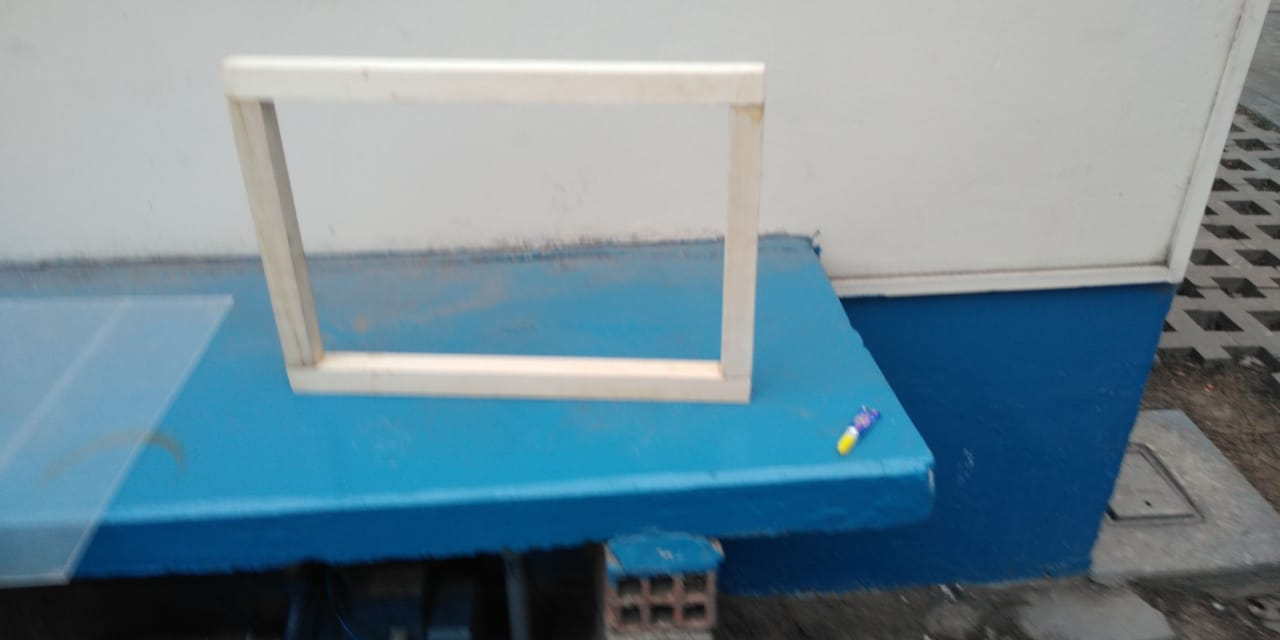
\includegraphics[scale=0.34]{mak.jpeg}
\caption[Maqueta]{Estructura de la maqueta antes de implementar los componentes electrónicos}
\end{center}
\end{figure}
\begin{figure}[H]
\begin{center}
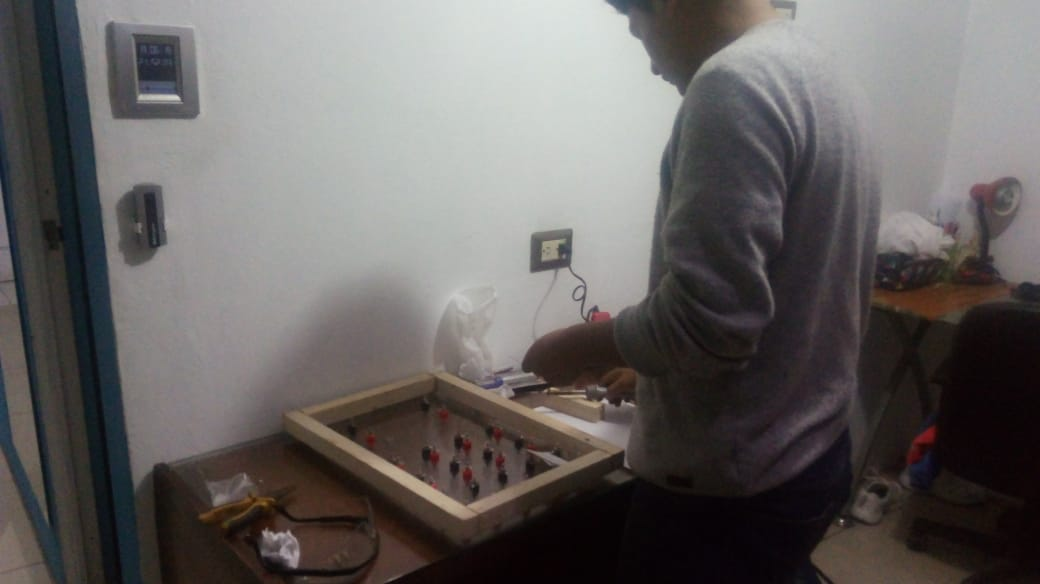
\includegraphics[scale=0.38]{kesk.jpeg}
\caption[Implementación de los componentes electrónicos]{Implementación de los componentes electrónicos}
\end{center}
\end{figure}
\begin{figure}[H]
\begin{center}
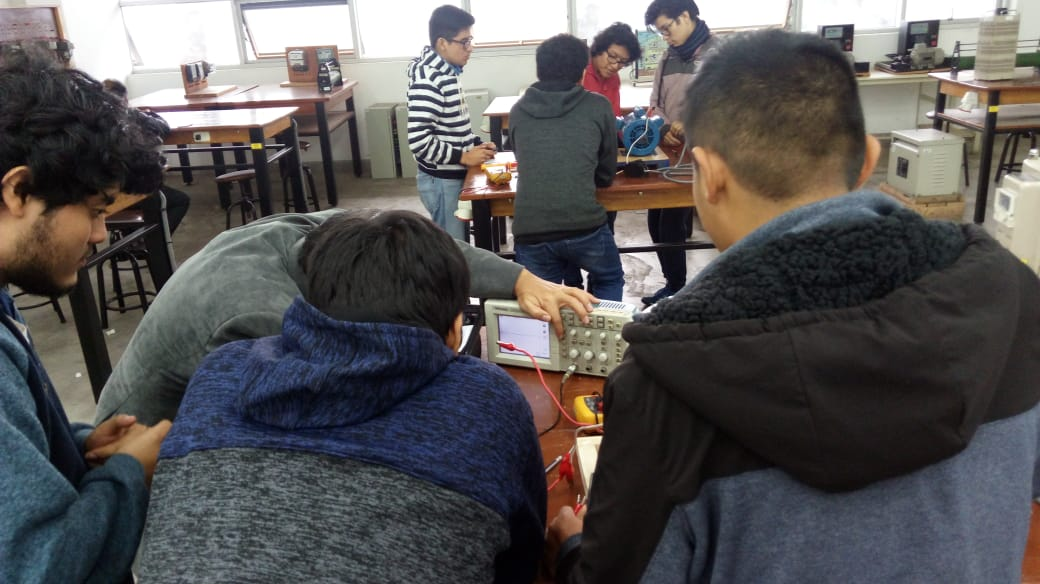
\includegraphics[scale=0.4]{iyo.jpeg}
\caption{Comprobación experimental de los resultados}
\end{center}
\end{figure}
\begin{figure}[H]
\begin{center}
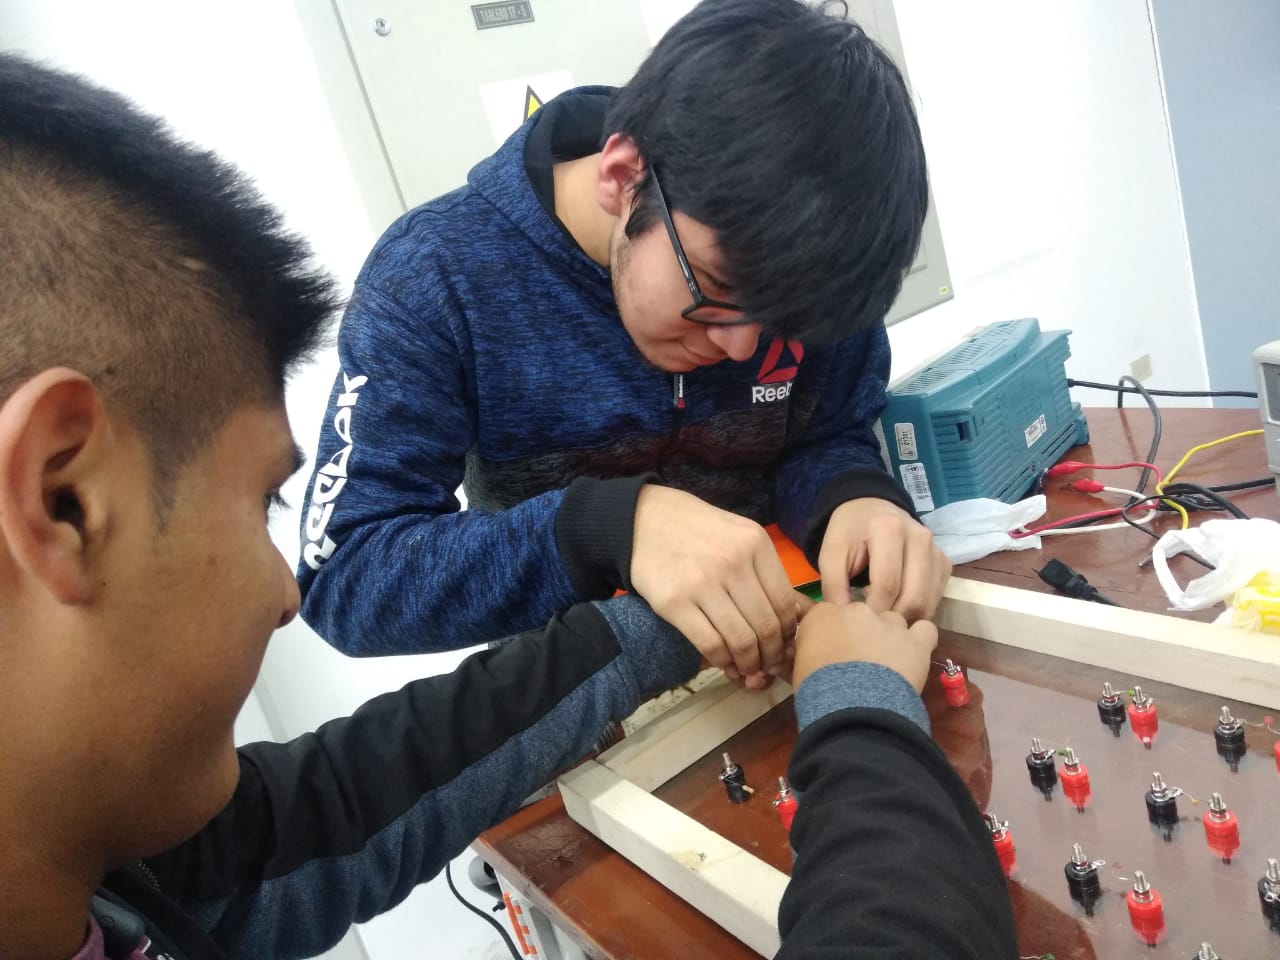
\includegraphics[scale=0.35]{serg.jpeg}
\caption{Rectificación de los resultados}
\end{center}
\end{figure}
\end{document}
